\section{Evaluation}
\label{sec:eval}

Once we obtain the cultural difference score of 
each English-Chinese term pair, we are able to sort them by decreasing
order. Our previous example of ``dragon'' and ``loong'' ranks 369 or
top 18.5\% among 2000 labeled pairs. 
Table \ref{tab:top10} shows the top 10 culturally different 
pairs discovered by cosine-knn method. To understand why
these terms have cultural differences, take ``amusement'' and ``娱乐'' for an
example. Table \ref{tab:nn} shows their top 5 nearest neighbors and we can find that ``amusement'' in English is more inclined to people's feeling, while ``娱乐'' in Chinese is usually related to the entertainment industry.  These results do show substantial 
differences in the context of their use. 

To determine the ground truth that a pair of terms is culturally 
different or not, we get help from Bing image search.
We believe that if an entity or object has cultural differences, such
differences should be reflected in people's general perception or 
images of the object, which are captured by large commercial search
engines such as Bing. This is evident from the images of 
dragon and loong in \figref{fig:dragon} and \figref{fig:loong}. 
In this section, we will discuss how we create the evaluation 
data set with Bing search and present the results.

\begin{table}
\small
\centering
\begin{tabular}{|c|c|c|c|c|c|}
\hline
 & English & Chinese &  & English & Chinese\\ \hline
\hline
1 & \bf{amusement} & \bf{娱乐} & 6 &  \bf{blade} &  \bf{叶片} \\
\hline
2 & \bf{cross} & \bf{十字架} & 7 &  \bf{raven} &  \bf{掠夺} \\
\hline
3 &  \bf{relief} &  \bf{浮雕} & 8 & \bf{regiment} &  \bf{团} \\
\hline
4 &  \bf{pitcher} &  \bf{投手} & 9 &  \bf{content} &  \bf{内容} \\
\hline
5 &  citation &  引用 & 10 &  \bf{review} &  \bf{回顾} \\

\hline
\end{tabular}
\caption{Top 10 culturally different words by cosine-knn (bold for culturally different pairs)}
\label{tab:top10}
\end{table}

\begin{table}
\small
\centering
\begin{tabular}{|c|c|c|}
\hline
 & \bf{amusement} & \bf{娱乐} \\ \hline
\hline
1 & pleasure & 投资 (investment) \\
\hline
2 & sympathy & 商业 (business)\\
\hline
3 &  humor & 购物 (shopping)\\
\hline
4 &  pride &  广告 (advertising)\\
\hline
5 &  enthusiasm &  产业 (industry)\\

\hline
\end{tabular}
\caption{5 nearest neighbors of ``amusement'' and ``娱乐'' by cosine-knn}
\label{tab:nn}
\end{table}

\subsection{Evaluation data}

We select the most common 2000 English terms (from our corpus)
along with their Chinese equivalents to form an evaluation data set. 
Human annotators are 
asked to search the English and Chinese word in Bing image 
search engine respectively and judge whether the results are visually
different.  For example, if you search the term ``dragon'' in English 
and ``loong'' in Chinese, you will find quite different images from
both queries. However, a search for ``computer'' and ``电脑'' yields
very similar images. 

\subsection{Results and Discussion}

\begin{figure*}[th]
\subfloat[Precision curve]{\label{fig:precision}
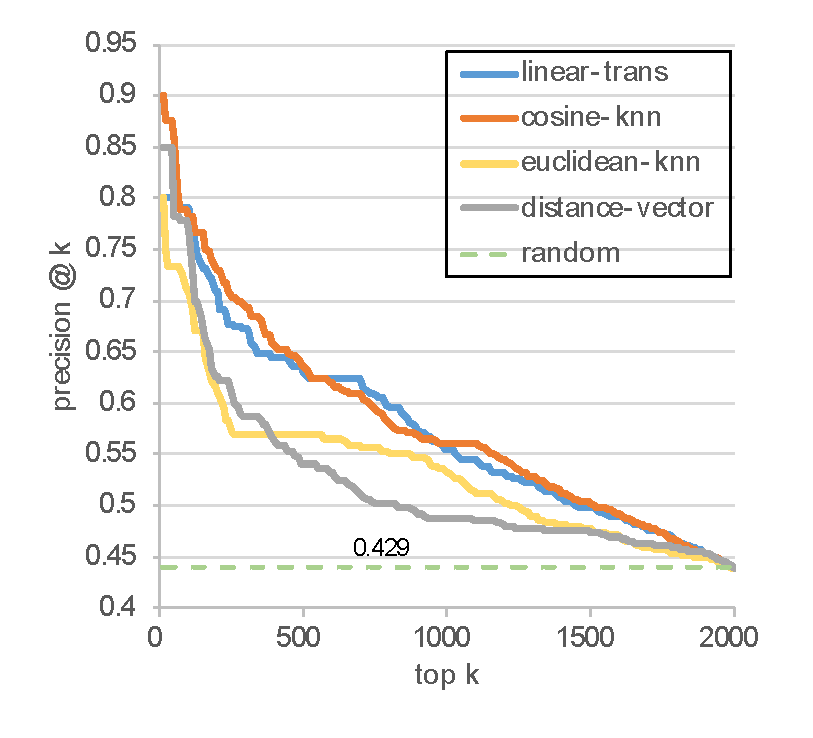
\includegraphics[width=0.32\textwidth]{img/precision}}\hfill
\subfloat[Recall curve]{\label{fig:recall}
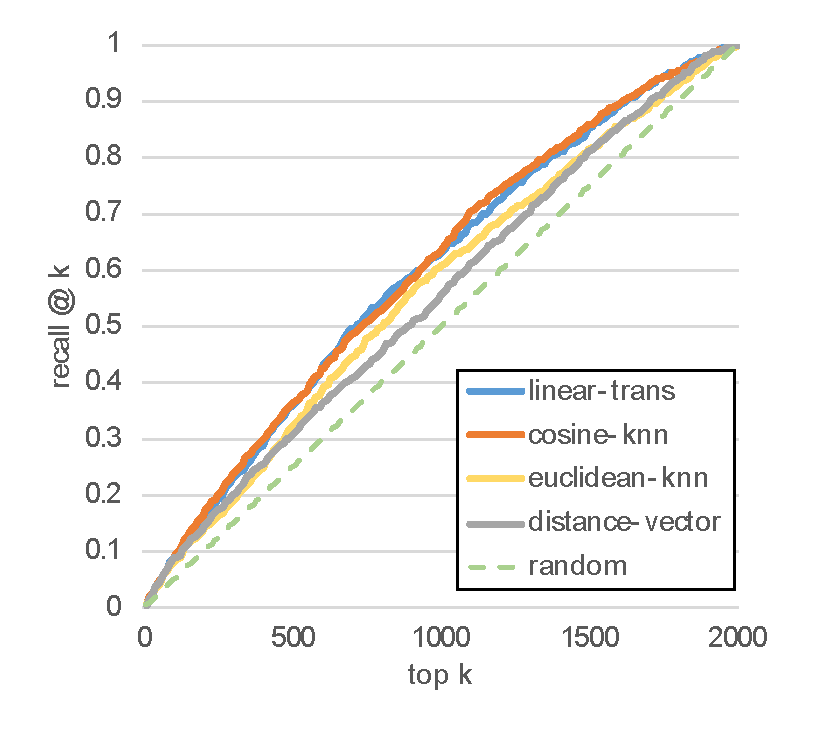
\includegraphics[width=0.32\textwidth]{img/recall}}\hfill
\subfloat[F1 curve]{\label{fig:f1}
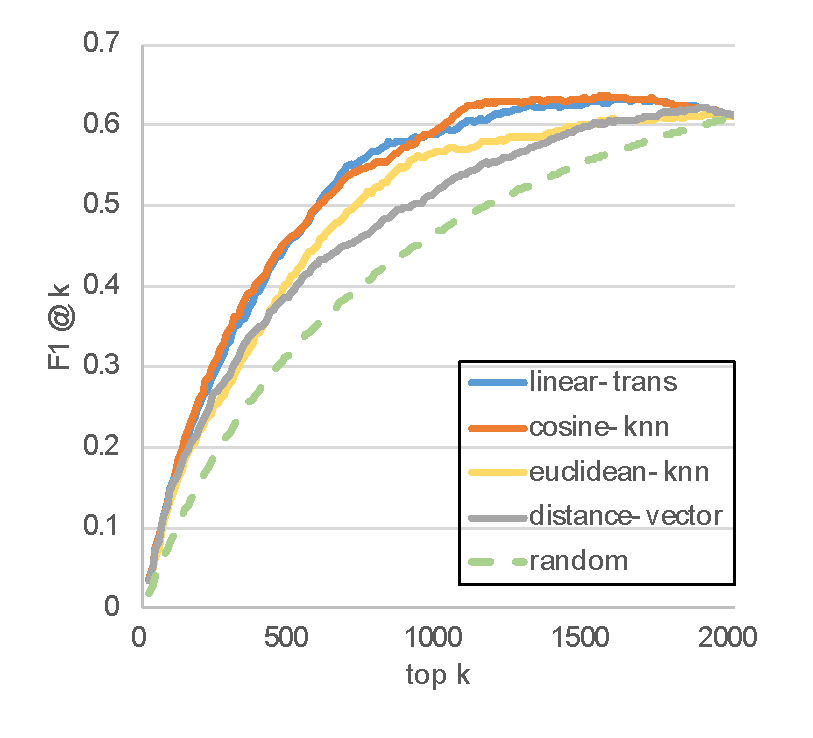
\includegraphics[width=0.32\textwidth]{img/F1}}
\caption{Precision, recall and F1-score for top $k$ pairs}
\label{fig:results}
\end{figure*}

As usual, we use precision, recall and F1 score to evaluate the 
top-k retrieval performance, as is shown in Figure \ref{fig:results} . We find that all of the four algorithms outperform the random baseline, which means our methodology captures 
cultural differences to varying degrees. Furthermore, 
cosine-knn algorithm performs better than other methods
for term pairs up to top 500, while the highest precision of
0.9 is achieved for top 10 pairs. 

To give an overall evaluation of our result, we also calculate the average precision of our four algorithms as follows: 

\begin{equation*}
 \operatorname{AvePrecision} = \frac{\sum_{k=1}^n (P(k) \times \operatorname{rel}(k))}{|\mbox{culturally different pairs}|} \!
\end{equation*}
where $P(k)$ represents the precision score at top $k$ and 
$\operatorname{rel}(k)$ is an indicator function equaling 1 if the item at rank k is culturally different,  zero otherwise. Table \ref{tab:ap} shows the average precision scores of our four algorithms and we can see the cosine-knn method has a notable advantage over the other three.
We think the reason why cosine-knn performs better is that it doesn't have any assumption for the relationship of different embedding spaces, which is the basics of linear transformation method. Meanwhile, cosine-knn is expressive enough as we tune the parameter $k$ and a tuned model is able to filter out the noises that bring down distance-vector method.
\begin{table}
\centering
\small
\begin{tabular}{|c|c|}
\hline
 & AvePrecision \\ \hline
 \hline
 linear-trans & 0.606 \\
 \hline
 cosine-knn & {\bf 0.617} \\
 \hline
 euclidean-knn & 0.579\\
 \hline
 distance-vector & 0.540\\ 
\hline
\end{tabular}
\caption{Average precision of 4 similarity calculation method}
\label{tab:ap}
\end{table}


